%  Preprint build for Zenodo: the same sections as main.tex (the MDPI MAKE submission), in a plain
%  layout with no journal branding, DOI, line numbers or submission status.
%  Build: pdflatex preprint && bibtex preprint && pdflatex preprint && pdflatex preprint
\documentclass[11pt,a4paper]{article}

\usepackage[T1]{fontenc}
\usepackage[utf8]{inputenc}
\usepackage{newpxtext,newpxmath}
\usepackage[margin=2.5cm]{geometry}
\usepackage{amsmath,graphicx,booktabs,tabularx,array,multirow,float,xcolor,subcaption,changepage}
\usepackage{tikz}
\usetikzlibrary{positioning, arrows.meta, shapes.geometric}
\usepackage[font=small,labelfont=bf]{caption}
\usepackage[numbers,sort&compress]{natbib}
\usepackage[hidelinks]{hyperref}
\usepackage{microtype}

% Macros the shared section files use from the MDPI class.
\newlength{\extralength}\setlength{\extralength}{1.23cm}
\newlength{\fulllength}\setlength{\fulllength}{18.46cm}
% Shared wide figures/tables retain the MDPI width, centred on the preprint page.
\let\preprintadjustwidth\adjustwidth
\let\endpreprintadjustwidth\endadjustwidth
\renewenvironment{adjustwidth}[2]{\preprintadjustwidth{#1}{#1}}{\endpreprintadjustwidth}
\setlength{\tabcolsep}{4pt}
\AddToHook{env/table/begin}{\let\small\footnotesize}
\makeatletter\newcommand{\rowsfrom}[1]{\@@input #1 }\makeatother
\graphicspath{{./}}

\title{\textbf{Scalable Extraction of Author-Stated Research Gaps:\\Towards Automated Idea Generation}}
\author{Yazan Alnakri$^{1}$, Osama Orabi$^{1,2}$ and Hamza Shafee Aldaghstany$^{1}$\\[4pt]
\normalsize $^{1}$Laboratory for Robotics and Artificial Intelligence, Innopolis University,\\\normalsize 420500 Innopolis, Russia\\
\normalsize $^{2}$Moscow Independent Research Institute of Artificial Intelligence (MIRAI),\\\normalsize 117218 Moscow, Russia\\[2pt]
\normalsize \texttt{\{y.alnakri, o.orabi, h.aldaghstany\}@innopolis.university}\\[2pt]
\small ORCID: Y.A.~\href{https://orcid.org/0009-0004-3990-5090}{0009-0004-3990-5090}, O.O.~\href{https://orcid.org/0009-0000-0028-315X}{0009-0000-0028-315X}, H.S.A.~\href{https://orcid.org/0009-0008-4938-2472}{0009-0008-4938-2472}}
\date{Preprint (v1), November 2026}

\begin{document}
\maketitle

\begin{abstract}
\noindent Papers state their own research gaps: limitations, future work and open problems. These statements could seed automated idea generation, but they are rare, scattered and easily confused with other text. Asking a large language model (LLM) to judge every sentence is costly, and giving it the whole paper buries the few relevant sentences. We instead narrow each paper with a funnel: rules discard unlikely text, a natural-language-inference classifier proposes candidates, and the LLM only verifies them. Every output is a sentence the authors wrote, and one instruction sets the verifier to favour precision or recall. We evaluate on human-labelled limitation (SAL) and future-work (FWS) benchmarks and on 230 LLM-labelled papers not yet checked by people. The instruction controlled the trade-off on every dataset, and verification more than doubled SAL precision at 85\% recall. In its cheapest variant (one call per paper, classifier fine-tuned on our LLM labels), the funnel reads 7--8 times fewer input tokens than whole-paper prompting and matches or improves \texorpdfstring{$F_1$}{F1} on both human-labelled benchmarks at every model size. Small models gain most: with a 4B LLM, \texorpdfstring{$F_1$}{F1} on arXiv rose from 0.30 to 0.48. With a 27B LLM, whole-paper prompting stayed ahead on arXiv.

\medskip\noindent\textbf{Keywords:} research gap extraction; limitations; future work; scientific text mining; large language models; natural language inference; zero-shot classification; LLM filtering
\end{abstract}

\section{Introduction}
\label{sec:introduction}

Research papers often say where a study falls short and what should be done next. Authors acknowledge the limitations of their own work, which tell readers how far its design, execution and interpretation limit the findings~\cite{kilicoglu2018automatic,lan2024automatic}. They propose future work that names the extensions and open questions they consider worth pursuing~\cite{zhu2019recognizing,zhang2023fws}, and they point to unsolved problems in their field when they motivate their own work. We call these statements \emph{author-stated research gaps}: limitations of the authors' own work, future-work directions they propose, and open problems they identify. Collected across many papers, they are a natural input for automated idea generation, because each one is a claim, made by a domain expert, about what is still missing.

Gap statements are hard to find for four reasons. They are rare: in the test sets we use, they make up 2.6\% of the sentences of randomized controlled trial (RCT) reports, 5.7\% of full arXiv and biomedical papers and 14.6\% of conclusion sections. They are scattered: a limitation may sit in a dedicated section, in the discussion or next to a methodological choice, and in computer-science papers many gaps appear in the methods and experiments sections. Many sentences look like gaps without being one, such as a criticism of prior work or a restated result. And the output must stay attributable: a system that writes plausible criticism answers a different question from one that finds what the authors actually wrote~\cite{xu2025llms,mishra2026tree}.

A large language model (LLM) can judge whether a sentence states a gap; the open question is how much of the paper to give it. Judging every sentence in a separate request is expensive. Giving the model the whole paper is simpler, but then a few relevant sentences sit among thousands to tens of thousands of tokens, and LLMs use information in the middle of long inputs less reliably~\cite{liu2024lost}, with accuracy falling as inputs grow~\cite{hsieh2024ruler}. This matters most for the smaller models that make processing large collections affordable.

Our idea is to shrink the LLM's job. Instead of asking it to find the gaps in a paper, we ask it only to verify a short list of candidates that cheaper components have already selected. Earlier extraction work points in the same direction: clinical limitation recognition uses section titles and limitation keywords to select candidate sentences, and these rules alone were more accurate than supervised classifiers~\cite{kilicoglu2018automatic}; future-work recognition separates locating sentences from grouping or classifying them~\cite{zhu2019recognizing,zhang2023fws}. We build this division of labour into a three-stage funnel (Figure~\ref{fig:pipeline-overview}). Stage~A removes text that is unlikely to contain gaps, Stage~B selects candidate sentences with a zero-shot natural-language-inference (NLI) classifier, and Stage~C asks an LLM to keep or drop each candidate. No stage rewrites text, so every output is a sentence the authors wrote. Stage~B needs no gap-labelled training data, so the same funnel runs on biomedical and computer-science papers. Because the LLM only verifies, its behaviour can also be steered with a single instruction: a mode paragraph in the system prompt sets Stage~C to high precision, balanced or high recall. A false gap wastes effort in idea generation, so precision is our primary goal and high precision is the main mode.

\begin{figure}[!htb]
\begin{adjustwidth}{-\extralength}{0cm}
\centering
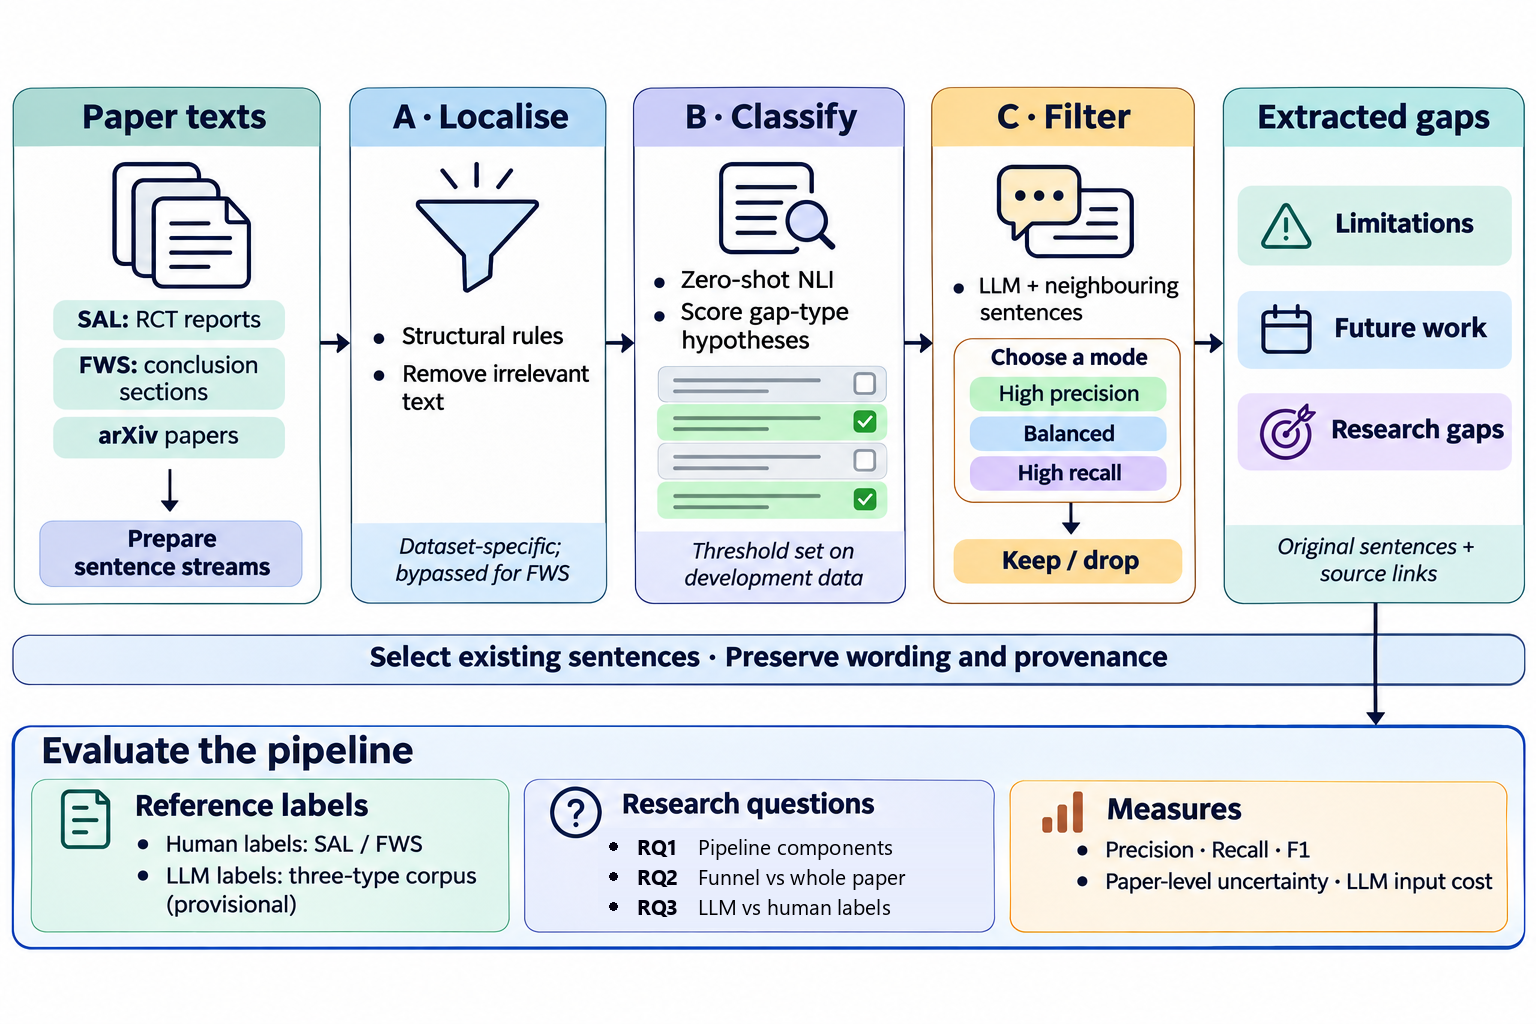
\includegraphics[width=\fulllength]{figures/gap2idea_graphical_abstract_v2.png}
\end{adjustwidth}
\caption{Overview of the funnel. Each paper is split into sentences. Stage~A removes text that is unlikely to contain gaps (its rules depend on the dataset; FWS skips it), Stage~B selects candidate sentences with a zero-shot NLI classifier, and Stage~C asks an LLM to keep or drop each candidate. The three filter modes are alternative instructions for Stage~C, not consecutive steps. Every output is an original sentence with its source. Evaluation uses human labels on SAL (limitations) and FWS (future work), and provisional LLM labels for all three gap types.\label{fig:pipeline-overview}}
\end{figure}

We evaluate the funnel on two benchmarks with human labels, self-acknowledged limitations in RCT reports (SAL)~\cite{lan2024automatic} and future-work sentences in natural language processing (NLP) papers (FWS)~\cite{zhang2023fws}. Each covers one gap type in one field, so we also built a corpus of 230 arXiv and biomedical papers in which two LLMs labelled all three gap types independently and an LLM judge resolved their disagreements. We compare the funnel with giving the same LLM the whole paper, using 27B, 9B and 4B models, and ask four questions:
\begin{itemize}
  \item \textbf{RQ1 (stages).} How much does each stage change precision and recall on full papers?
  \item \textbf{RQ2 (precision control).} Does one instruction set the precision--recall trade-off of the LLM filter consistently across datasets?
  \item \textbf{RQ3 (whole-paper prompting).} How does the funnel compare with giving the same LLM the whole paper, in accuracy and cost, and does the answer depend on the size of the LLM?
  \item \textbf{RQ4 (classifier).} Is a training-free classifier enough for Stage~B, compared with a classifier trained on human labels or one fine-tuned on our LLM labels?
\end{itemize}

Narrowing the LLM's job pays off most where the LLM is weakest. With a 4B model, whole-paper prompting kept most sentences of several long arXiv papers. The funnel, sending each paper's candidates in a single call with the Stage~B classifier fine-tuned on our LLM labels, raised $F_1$ on arXiv from 0.30 to 0.48 while the LLM read about seven times fewer input tokens (Tables~\ref{tab:wholecost} and~\ref{tab:variants}). With a 27B model, the two approaches are closer: the funnel scores higher on the human-labelled benchmarks with less input, and whole-paper prompting scores higher on arXiv papers, whose labels were themselves made from whole papers. Our contributions are:
\begin{enumerate}
  \item \textbf{A source-preserving funnel for gap extraction} in which the LLM only verifies candidates, every output is an author-written sentence, and one instruction sets the trade-off between precision and recall. The modes kept their order on every dataset; in high-precision mode, verification raised precision on SAL from 29.1\% to 66.2\% at 84.9\% recall (Sections~\ref{sec:rq1} and~\ref{sec:rq2}).
  \item \textbf{A comparison with whole-paper prompting across three LLM sizes}, in accuracy and cost. On full papers, the funnel reads about 7--8 times fewer input tokens in its one-call-per-paper format, and its advantage grows as the model gets smaller (Sections~\ref{sec:rq3} and~\ref{sec:format}).
  \item \textbf{An analysis of the stages and of the classifier.} Stage~A helps where section headings are informative, Stage~B sets the recall ceiling because Stage~C can only remove candidates, and Stage~C supplies most of the precision gain on full papers. A zero-shot classifier comes within 0.021 $F_1$ of a supervised one on SAL, at lower precision (Section~\ref{sec:rq4}).
  \item \textbf{A three-type evaluation corpus and two evaluation pitfalls.} We release the LLM-labelled corpus with every LLM verdict behind our results. We also show that the same SAL output has 66.2\% precision against human labels and 93.2\% against LLM labels, and that letter case reveals the label in the public FWS corpus, so we lowercase all FWS text (Sections~\ref{sec:label-source} and~\ref{sec:fws-case}).
\end{enumerate}

The scope of this paper is extraction. Whether an extracted gap is still open, and whether it leads to a useful research idea, are separate questions. Section~\ref{sec:related} reviews related work. Section~\ref{sec:methods} describes the data, the funnel and the comparisons. Section~\ref{sec:results} reports the results, Section~\ref{sec:discussion} discusses them and the limitations of the study, and Section~\ref{sec:conclusions} concludes.

\section{Related Work}
\label{sec:related}

Our task connects the recognition of author-stated limitations and future work with rhetorical sentence classification and with LLM-based processing of scholarly text. These areas share input documents and some methods, but their output claims differ. Table~\ref{tab:related} summarises the studies closest to ours.

\subsection{Rhetorical annotation and scientific sentence classification}

Argumentative zoning classifies sentences by their role in a scientific argument~\cite{teufel2002summarizing}, and later schemes such as Core Scientific Concepts add categories related to gaps, failures and future work~\cite{liakata2010corpora}. The Dr.~Inventor corpus annotates limitations and future work in separate layers of 40 full articles~\cite{fisas2016multilayered}. Abstract-level resources such as PubMed 200k RCT, CSAbstruct, MAZEA and Emerald~110k broaden the available schemes~\cite{dernoncourt2017pubmed,cohan2019pretrained,dayrell2012rhetorical,stead2019emerald}, but an abstract role such as conclusion does not tell whether a sentence states a gap. Context helps classify short sentences: hierarchical and cross-domain models use surrounding sentences~\cite{jin2018hierarchical,brack2024sequential}, LLMs have been applied to multi-label sentence classification~\cite{lan2024multilabel}, and context-enhanced models extract problem and method sentences~\cite{zhang2024extracting}. Our filter also gives the LLM neighbouring sentences, but only to judge a candidate, not to label every sentence of a paper.

\subsection{Author-stated limitations and future work}

Kilicoglu et al.~\cite{kilicoglu2018automatic} recognise self-acknowledged limitations in clinical research with section rules and learned classifiers; their use of headings to narrow the search is a direct precedent for our Stage~A. Lan et al.~\cite{lan2024automatic} annotate 200 RCT publications (SAL) and fine-tune PubMedBERT for limitation detection and typing, reporting a binary detection $F_1$ of 0.821 on a section-filtered candidate pool. That pool and its positive rate differ from the full-paper stream we score, so the numbers are not directly comparable. For future work, Zhu et al.~\cite{zhu2019recognizing} recognise future-research sentences in JASIST articles and cluster them, the ACL FWS-RC corpus provides future-work labels and a taxonomy~\cite{hao2020acl}, and Zhang et al.~\cite{zhang2023fws} report recognition and classification results on it (macro-$F_1$ 0.907 for recognition). Suray et al.~\cite{suray2024future} trace whether later work engages with future-work statements, a downstream use of extraction.

\subsection{LLM extraction, inferred gaps and generated critique}

Several recent studies use LLMs on related tasks. LimGen collects author-written limitation sections from 4068 ACL papers to generate suggested limitations~\cite{faizullah2024limgen}. BAGELS combines parsing and LLM processing to extract and generate limitations across NLP, machine learning and biology~\cite{alazher2025bagels}, and FutureGen extracts future-work statements and then generates new ones with retrieval augmentation~\cite{alazher2025futuregen}. GAPMAP separates explicitly stated knowledge gaps from gaps inferred from context in biomedical text~\cite{salem2025gapmap}. LimitGen and Tree-of-Concerns ask models to find limitations that authors did not state~\cite{xu2025llms,mishra2026tree}. In these works the LLM often generates text; in ours it only accepts or rejects a sentence the authors wrote. Sci-Sentence labels research gaps and limitations among seven rhetorical roles in literature reviews~\cite{bolanos2025scisentence}; its research-gap class is close to our third type, but its sentences come from review sections rather than full papers.

\subsection{Position of this work}

Structural filtering, learned classifiers and LLM judgement each have precedents. What we add is a measured combination of the three on full-paper sentence streams, a training-free Stage~B that transfers across domains, an explicit control of the LLM filter's precision--recall trade-off, and an evaluation that keeps label source, dataset and processing unit separate.

\begin{table}[H]
\caption{Selected related work, ordered by year. ``Unit'' is the input each method processes.\label{tab:related}}
\begin{adjustwidth}{-\extralength}{0cm}
\footnotesize
\setlength{\tabcolsep}{3pt}
\begin{tabularx}{\fulllength}{@{}>{\raggedright\arraybackslash}p{2.9cm}>{\raggedright\arraybackslash}p{2.4cm}>{\raggedright\arraybackslash}p{2.2cm}>{\raggedright\arraybackslash}p{3.2cm}>{\raggedright\arraybackslash}p{1.8cm}>{\raggedright\arraybackslash}X@{}}
\toprule
\textbf{Study} & \textbf{Domain} & \textbf{Statement type} & \textbf{Approach} & \textbf{Unit} & \textbf{Relation to this study}\\
\midrule
Dr.~Inventor, 2016~\cite{fisas2016multilayered} & Computer graphics & Limitations; future work & Human multi-layer annotation & Sentences, full articles & Full-text precedent with both statement types\\
Kilicoglu et al., 2018~\cite{kilicoglu2018automatic} & Clinical research & Limitations & Rules; supervised classifiers & Sentences & Precedent for section-based localisation\\
Zhu et al., 2019~\cite{zhu2019recognizing} & Information science & Future work & BERT classification; clustering & Sentences, full articles & Links recognition to thematic analysis\\
ACL FWS-RC, 2020~\cite{hao2020acl} & NLP & Future work & Annotation; taxonomy & Sentences & Source of FWS labels\\
Zhang et al., 2022~\cite{zhang2023fws} & NLP & Future work & Lexical and neural recognition & Sentences & FWS recognition benchmark\\
LimGen, 2024~\cite{faizullah2024limgen} & NLP & Limitations & LLM generation & Paper & Author limitation sections as references\\
Lan et al., 2024~\cite{lan2024automatic} & RCT reports & Limitations & PubMedBERT detection and typing & Sentences & Source of SAL; supervised comparison\\
Lan et al., 2024~\cite{lan2024multilabel} & Several sciences & Rhetorical roles & LLM prompting and fine-tuning & Abstract sequence & Context-aware LLM labelling\\
Zhang \& Zhang, 2024~\cite{zhang2024extracting} & NLP & Problem; method & Context-enhanced transformer & Sentence with context & Local context for sparse targets\\
Brack et al., 2024~\cite{brack2024sequential} & Several sciences & Rhetorical roles & Cross-domain multi-task learning & Sentence sequence & Transfer across domains\\
Suray et al., 2024~\cite{suray2024future} & Usable security & Future work & Statement and citation analysis & Statement & Downstream use of extracted directions\\
BAGELS, 2025~\cite{alazher2025bagels} & NLP; ML; biology & Limitations & Parsing; LLM extraction and generation & Paper & Closest extraction precedent\\
FutureGen, 2025~\cite{alazher2025futuregen} & NLP; ML & Future work & LLM extraction; RAG generation & Paper & Extraction feeding generation\\
GAPMAP, 2025~\cite{salem2025gapmap} & Biomedicine & Knowledge gaps & LLM detection and inference & Paragraph to paper & Explicit versus inferred gaps\\
LimitGen, 2025~\cite{xu2025llms} & AI & Limitations & LLM and agent evaluation & Paper & Unstated limitations; different target\\
Sci-Sentence, 2025~\cite{bolanos2025scisentence} & Literature reviews & Research gap; limitation & Encoder and LLM classifiers & Sentence & Research-gap label close to ours\\
Tree-of-Concerns, 2026~\cite{mishra2026tree} & ML; NLP; vision & Limitations & Multi-agent critique & Paper & Unstated critique; different target\\
\midrule
\textbf{This study} & RCT reports; NLP; arXiv & Limitations; future work; research gaps & Rules, zero-shot NLI, LLM filter with three modes & Sentence with context & Measures stage contribution, precision control and cost\\
\bottomrule
\end{tabularx}
\end{adjustwidth}
\end{table}

\section{Materials and Methods}
\label{sec:methods}

Figure~\ref{fig:pipeline-overview} summarises the extraction workflow and its evaluation. The following subsections define the targets, data, processing stages and evaluation protocol.

\begin{figure}[htbp]
\begin{adjustwidth}{-\extralength}{0cm}
\centering
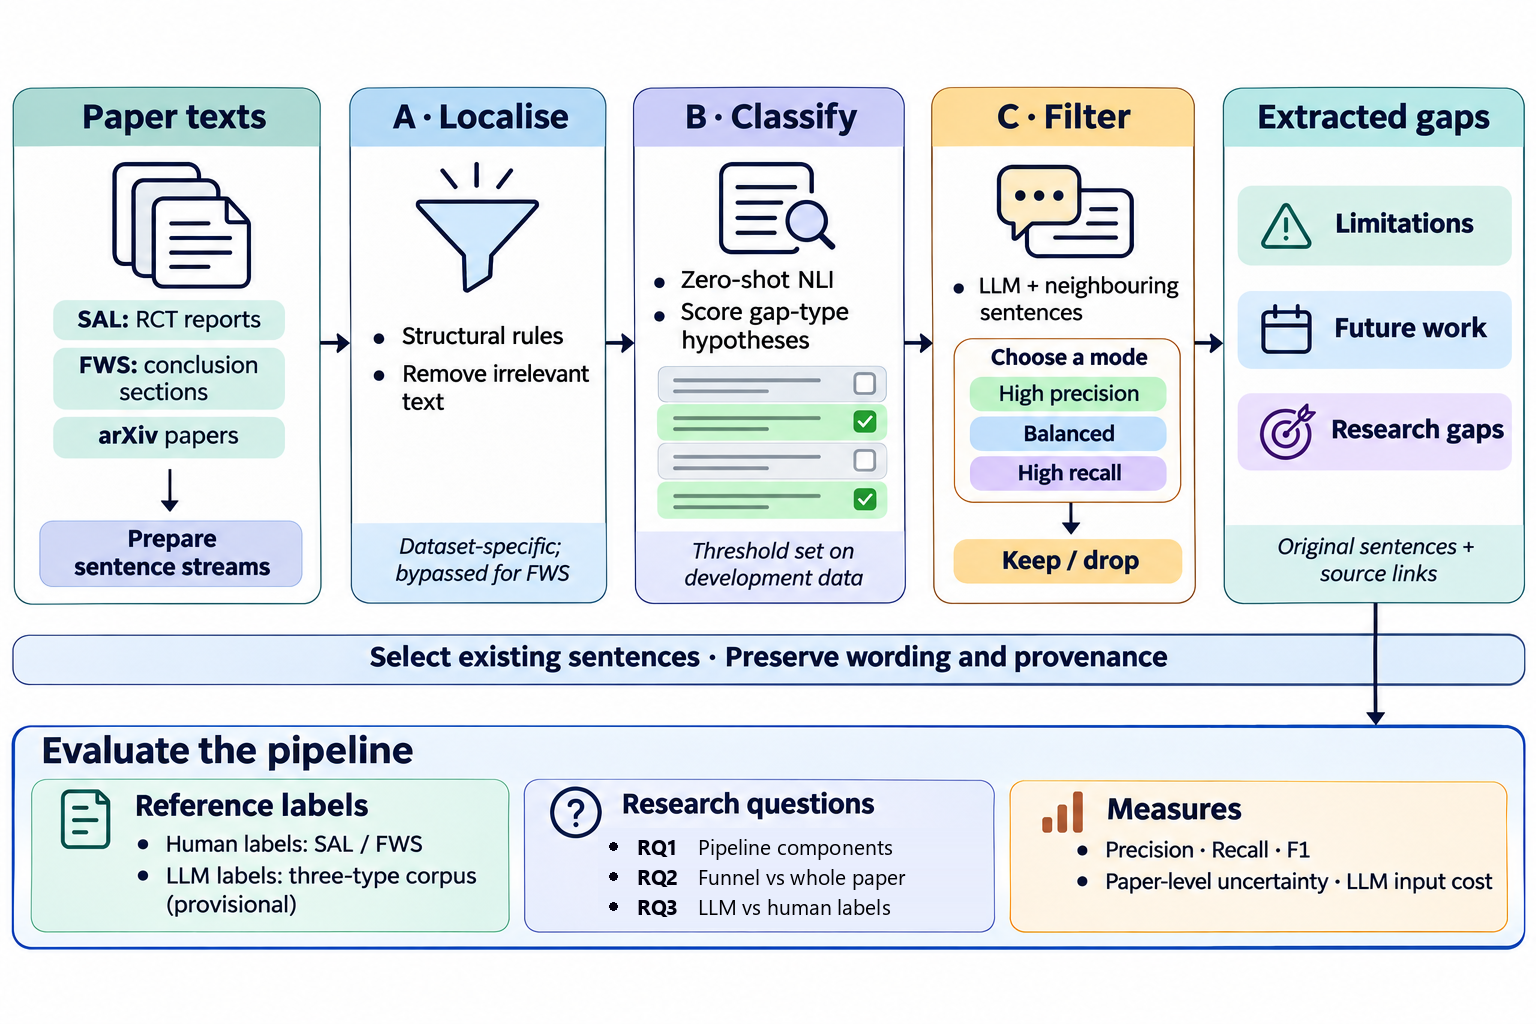
\includegraphics[width=\fulllength]{figures/gap2idea_graphical_abstract_v2.png}
\end{adjustwidth}
\caption{Overview of Gap2Idea. Paper texts are prepared as sentence streams, then processed by structural localisation (A), zero-shot NLI candidate selection (B) and an LLM filter (C). The three filter modes are alternative settings. Outputs retain the original wording and source identifiers. Stage~A is dataset-specific and bypassed for FWS. Human-labelled SAL and FWS evaluate limitations and future work, respectively; evaluation of all three types uses provisional LLM labels. Stage contributions, precision--recall control and classifier choice are assessed alongside LLM input cost.\label{fig:pipeline-overview}}
\end{figure}

\subsection{Task}

The input is the sentence stream of a full paper. The output is the set of sentences that state an author-stated research gap of one of three types:
\begin{itemize}
  \item \textbf{Limitation}: a weakness, caveat, bias, constraint or assumption the authors acknowledge about their own work;
  \item \textbf{Future work}: an explicit direction the authors propose for future research;
  \item \textbf{Research gap}: an unsolved problem, missing capability or open challenge the authors point to in the field or in prior work.
\end{itemize}
Each output is an unmodified source sentence. Scoring is binary at the sentence level: a predicted sentence is correct if its label is any gap type covered by the benchmark. SAL labels only limitations and FWS only future work, so on those benchmarks the funnel targets that one type.

\subsection{Data}

Table~\ref{tab:data} summarises the evaluation data. All splits are by paper.

\begin{table}[htbp]
\caption{Evaluation data. Positives are sentences labelled with a gap type the benchmark covers.\label{tab:data}}
\begin{adjustwidth}{-\extralength}{0cm}
\small
\begin{tabularx}{\fulllength}{@{}>{\raggedright\arraybackslash}p{3.0cm}>{\raggedright\arraybackslash}p{2.3cm}>{\raggedright\arraybackslash}p{2.6cm}rrr>{\raggedright\arraybackslash}X@{}}
\toprule
\textbf{Dataset (split)} & \textbf{Labels} & \textbf{Gap types} & \textbf{Papers} & \textbf{Sentences} & \textbf{Positives} & \textbf{Use}\\
\midrule
SAL (test) & Human & Limitation & 40 & 7968 & 205 & Main evaluation\\
SAL (dev) & Human & Limitation & 40 & 7729 & 180 & Threshold; held-out check\\
FWS (test) & Human & Future work & 209 & 1506 & 220 & Evaluation\\
FWS (dev) & Human & Future work & 418 & 3005 & 418 & Threshold\\
Gold corpus (test) & LLM ensemble & All three & 34 & 11,741 & 664 & Evaluation\\
Gold corpus (validation) & LLM ensemble & All three & 34 & 11,201 & 699 & Design choices; thresholds\\
\bottomrule
\end{tabularx}
\end{adjustwidth}
\end{table}

\paragraph{SAL.} SAL contains 200 RCT publications with sentence-level limitation labels, split into 120 training, 40 development and 40 test papers~\cite{lan2024automatic,salrepo}. We use full papers, not a section-filtered pool. Section types were recovered by matching each sentence to the PubMed Central BioC version of its article, and sentences of fewer than three words were removed; none of the removed test sentences is a limitation. The training split is used only to train the supervised comparison classifiers.

\paragraph{FWS.} The FWS recognition corpus holds conclusion-section sentences from ACL papers labelled as future work or not~\cite{hao2020acl,zhang2023fws,fwsrepo}. Because it contains conclusion sections only, it has no full-paper structure. We use a fixed test sample of 209 papers (1506 sentences) and a development sample of the next 418 papers in the same random order, after removing sentences that appear in an earlier training set of ours. In this corpus every positive sentence is entirely lowercase and almost no negative is (Section~\ref{sec:fws-case}), so we lowercase all FWS text before any processing.

\paragraph{Gold corpus.} We built a three-type corpus of 230 papers and 68,719 sentences: 190 arXiv computer-science and machine-learning papers, converted from PDF with PyMuPDF and split into sentences after removing reference lists, and the 40 SAL test papers with their original sentence boundaries. Two LLMs, Claude Opus~5.5 and Claude Sonnet~5.5, each labelled every sentence of every paper in one call per paper, following a written guideline with the three definitions above. Sentences marked by both with the same type form the high-confidence tier (2960 sentences). The other 1737 candidates marked by only one model, or with different types, were adjudicated by Claude Opus~5.5 with $\pm$3 sentences of context, which confirmed 1502. The final corpus has 4462 gap sentences: 2234 research gaps, 1543 limitations and 685 future-work statements. Agreement between the two labelling models on whether a sentence is a gap was $\kappa = 0.778$~\cite{cohen1960kappa}; this is agreement between models, not with humans. On the 40 SAL papers, the ensemble labelled all but nine of SAL's 205 human-labelled limitations as a gap. SAL labels were not shown to the labelling models. Papers were split into 162 training, 34 validation and 34 test papers. The test split has 664 gaps (220 limitations, 97 future work, 347 research gaps); 28 test papers are arXiv (527 gaps) and 6 are SAL papers (137 gaps). Labelling cost about US\$36.

\subsection{The funnel}

Figure~\ref{fig:funnel} shows the three stages and the gold-test counts at each.

\begin{figure}[htbp]
\begin{adjustwidth}{-\extralength}{0cm}
\centering
\begingroup
\definecolor{funnelInk}{HTML}{183249}
\definecolor{funnelInput}{HTML}{527385}
\definecolor{funnelA}{HTML}{147C87}
\definecolor{funnelB}{HTML}{6553A0}
\definecolor{funnelC}{HTML}{A66916}
\begin{tikzpicture}[
  x=1cm, y=1cm,
  font=\small, text=funnelInk,
  card/.style={rounded corners=5pt, line width=0.7pt},
  title/.style={font=\small\bfseries, anchor=north},
  detail/.style={font=\footnotesize, align=center},
  count/.style={font=\Large\bfseries},
  arr/.style={-{Stealth[length=2.4mm,width=1.8mm]}, line width=1pt, draw=funnelInput}]
% Native vector cards preserve legibility at print resolution.
\draw[card,draw=funnelInput!65,fill=funnelInput!5] (0,0) rectangle (3.1,-4.1);
\draw[card,draw=funnelA!65,fill=funnelA!6] (3.75,0) rectangle (6.85,-4.1);
\draw[card,draw=funnelB!65,fill=funnelB!6] (7.5,0) rectangle (10.6,-4.1);
\draw[card,draw=funnelC!65,fill=funnelC!6] (11.25,0) rectangle (17.6,-4.1);

\node[title,text=funnelInput] at (1.55,-0.23) {INPUT};
\node[title,text=funnelA] at (5.3,-0.23) {A. LOCALISE};
\node[title,text=funnelB] at (9.05,-0.23) {B. CLASSIFY};
\node[title,text=funnelC] at (14.425,-0.23) {C. FILTER};
\node[detail] at (1.55,-0.91) {Full-paper sentences};
\node[detail] at (5.3,-0.91) {Structural rules};
\node[detail] at (9.05,-0.91) {Zero-shot NLI};
\node[detail] at (14.425,-0.91) {LLM with neighbouring sentences};

\node[count,text=funnelInput] at (1.55,-1.67) {11,741};
\node[count,text=funnelA] at (5.3,-1.67) {9604};
\node[count,text=funnelB] at (9.05,-1.67) {2522};
\node[detail] at (1.55,-2.13) {input sentences};
\node[detail] at (5.3,-2.13) {sentences kept};
\node[detail] at (9.05,-2.13) {candidates kept};
\node[count,text=funnelInput] at (1.55,-2.83) {664};
\node[count,text=funnelA] at (5.3,-2.83) {644};
\node[count,text=funnelB] at (9.05,-2.83) {606};
\node[detail] at (1.55,-3.27) {labelled gaps};
\node[detail] at (5.3,-3.27) {labelled gaps retained};
\node[detail] at (9.05,-3.27) {labelled gaps retained};

% Alternative settings, each applied to the same Stage B candidates.
\node[anchor=west,font=\footnotesize\bfseries] at (11.53,-1.52) {Mode};
\node[font=\footnotesize\bfseries] at (15.12,-1.52) {Kept};
\node[font=\footnotesize\bfseries] at (16.78,-1.52) {Gaps};
\fill[rounded corners=3pt,funnelA!13] (11.45,-1.86) rectangle (17.4,-2.43);
\fill[rounded corners=3pt,funnelB!12] (11.45,-2.56) rectangle (17.4,-3.13);
\fill[rounded corners=3pt,funnelC!15] (11.45,-3.26) rectangle (17.4,-3.83);
\node[anchor=west,font=\footnotesize\bfseries,text=funnelA] at (11.6,-2.145) {High precision};
\node[anchor=west,font=\footnotesize\bfseries,text=funnelB] at (11.6,-2.845) {Balanced};
\node[anchor=west,font=\footnotesize\bfseries,text=funnelC] at (11.6,-3.545) {High recall};
\foreach \y/\kept/\gaps in {-2.145/440/381,-2.845/776/529,-3.545/1011/569} {
  \node[font=\small\bfseries] at (15.12,\y) {\kept};
  \node[font=\small\bfseries] at (16.78,\y) {\gaps};
}
\draw[arr] (3.13,-2.05) -- (3.71,-2.05);
\draw[arr] (6.88,-2.05) -- (7.46,-2.05);
\draw[arr] (10.63,-2.05) -- (11.21,-2.05);
\end{tikzpicture}
\endgroup
\end{adjustwidth}
\caption{Sentence selection on the gold test split (34 papers, provisional LLM labels). The first three cards show the input and the sentences retained after Stages~A and~B. Stage~C applies each alternative filter mode to the same candidates; ``Kept'' counts all selected sentences and ``Gaps'' counts selected sentences labelled as gaps. Each stage preserves the original text.\label{fig:funnel}}
\end{figure}

\paragraph{Stage A: localisation.} For SAL, Stage~A keeps sentences in Discussion and Conclusion sections, which retains 203 of 205 test limitations while removing 76.3\% of sentences. For the gold corpus, Stage~A is a rule-based junk filter with no section gate: it drops titles, tables, figure captions, abbreviation lists, competing-interest, author-contribution, funding and supplementary sections where section types are known, bibliography-like strings, and implausible sentences (under 25 characters or six tokens, starting mid-word, dot leaders, or mostly non-letters). A section gate is not used for arXiv papers because their gaps are spread through the body (Section~\ref{sec:discussion}). FWS has no Stage~A: it already consists of conclusion sections, and our junk filter, which rejects sentences that start in lower case, would reject almost all FWS text once it is lowercased.

\paragraph{Stage B: zero-shot NLI classifier.} Each sentence is scored by an NLI cross-encoder, ModernBERT-large fine-tuned on NLI data~\cite{warner2024modernbert,modernbertnli} (revision \texttt{ca476cb9}), used as a zero-shot classifier~\cite{yin2019zeroshot}. The sentence is the premise and a short hypothesis states the gap type: ``This is a limitation.'', ``This is future work.'' or ``This is a research gap.'' The score is the entailment probability divided by the sum of the entailment and contradiction probabilities. On the gold corpus a sentence is a candidate if its maximum score over the three hypotheses reaches a threshold $\tau$, and its predicted type is the hypothesis with the highest score. On SAL only the limitation hypothesis is used, and on FWS only the future-work hypothesis. Inputs are truncated to 256 tokens.

\paragraph{Stage C: LLM filter.} Candidates are sent in reading order, 20 per request, to Qwen3.8-27B (FP8, revision \texttt{017b9c7a}), self-hosted with vLLM~\cite{kwon2023vllm}. This model played no part in making any labels. Each item contains the predicted type, the sentence (up to 400 characters) and its context, the previous and next sentence of the same paper (up to 600 characters). The model returns a keep or drop verdict for each item as JSON constrained by a schema. Decoding uses temperature 0, seed 0 and no reasoning mode. The system prompt (Appendix~\ref{app:prompts}) gives the three definitions, a list of sentence kinds to drop (results, method descriptions, contribution claims, background, citations, captions and similar), and a final instruction that sets the mode:
\begin{itemize}
  \item \textbf{High recall}: when genuinely uncertain, keep the sentence;
  \item \textbf{Balanced}: favour neither keeping nor dropping;
  \item \textbf{High precision}: keep a sentence only if it explicitly states the gap itself, drop general background, motivation, observed outcomes and passing remarks, and when uncertain, drop it.
\end{itemize}
For SAL and FWS the definitions are narrowed to the benchmark's single type, and the other two types are added to the drop list. The wording of each mode is otherwise identical across datasets.

\subsection{How design choices were made}

Because several choices were tuned, we record where each was made.
\begin{itemize}
  \item \textbf{NLI hypotheses.} Hypothesis variants (long definitions, short type names, a single combined hypothesis, adding context, competing negative hypotheses) were compared on one half of the gold validation papers and confirmed on the other half. Short type names were best; context and negative hypotheses hurt.
  \item \textbf{Thresholds.} $\tau$ is the highest value whose overall recall, counting sentences lost in Stage~A, is at least 90\% on development data: gold validation ($\tau = 0.354$), SAL dev ($\tau = 0.7286$) and FWS dev ($\tau = 0.1922$). Values are rounded; at the rounded SAL value one development limitation falls below the threshold, so SAL dev recall before Stage~C is 89.4\% rather than 90.0\%.
  \item \textbf{Stage C model and rubric.} The model, batch size, use of context and the high-recall rubric were chosen during development using 196 candidates from gold test papers; we report gold results with and without these sentences. The balanced and high-precision wording was written after reading false positives from a high-recall run on gold test papers, and was then checked on the gold validation split before any further test run. All three modes were run on every test set and are reported, so no mode was selected by its test score.
  \item \textbf{Held-out check.} The SAL dev papers were used only to set $\tau$; no prompt was written or chosen on them. We run the full funnel on them as a check on unseen papers.
\end{itemize}

\subsection{Comparison systems}

\paragraph{Supervised classifiers on SAL.} We trained eight classifiers on the SAL training split: three fine-tuned encoders, PubMedBERT~\cite{gu2021pubmedbert} (\texttt{BiomedNLP-BiomedBERT-base-uncased-abstract-fulltext}), SciBERT~\cite{beltagy2019scibert} and DistilBERT~\cite{sanh2019distilbert}, each trained for three epochs (learning rate $3\times10^{-5}$, batch 32, class-weighted loss) with a threshold chosen on the SAL dev split; and five frozen sentence encoders~\cite{reimers2019sentencebert,xiao2023cpack} with logistic regression. PubMedBERT was the strongest and serves as the supervised Stage~B comparison; it is also the model family used by Lan et al.~\cite{lan2024automatic}.

\paragraph{Other Stage B options on the gold corpus.} A frozen bge-small encoder~\cite{xiao2023cpack} with a logistic-regression head trained on the gold training split, and the same ModernBERT NLI model with a single long hypothesis covering all gap types (threshold 0.75 chosen on validation).

\paragraph{Whole-paper LLM prompting and published methods.} Comparisons with whole-paper and every-sentence LLM prompting on the same test papers, and reproductions of published methods, are in progress and are not reported in this version.

\subsection{Evaluation}

We report positive-class precision, recall and $F_1$ at the sentence level. The recall denominator is every positive sentence in the test papers, including those removed by Stage~A. Confidence intervals (CIs) are 95\% percentile intervals from 2000 bootstrap resamples of papers~\cite{efron1993bootstrap}, since sentences from one paper are not independent. Comparisons between two systems are paired: both are scored on the same resampled papers, and we report the interval of the difference. LLM input cost is estimated with the \texttt{cl100k\_base} tokenizer~\cite{tiktoken} on the prompts and items exactly as sent; output tokens and Stage~A and B computation are excluded. For comparison we count the input of one whole-paper call (the high-precision prompt followed by the numbered sentences) and of judging every sentence in batches of 20 in the funnel's format. We measured run-to-run stability by repeating the high-recall run on the gold test candidates.

\subsection{Software and use of generative AI}

Experiments used Python with PyTorch, Hugging Face Transformers, sentence-transformers, scikit-learn and vLLM; exact versions are pinned in the repository's lock file. Code is available at the repository listed in the Data Availability Statement. Generative AI is part of the method in two places: Claude Opus~5.5 and Claude Sonnet~5.5 produced the gold-corpus labels, and Qwen3.8-27B is the Stage~C filter. Use of AI assistance in preparing the study and manuscript is declared in the Acknowledgments.

\section{Results}
% TODO: port from origin/paper-writing:manuscript/sections/

\section{Discussion}
\label{sec:discussion}

We first interpret the answers to the research questions. We then discuss when whole-paper prompting is enough, how reliable the extracted gaps are, why section rules do not transfer to computer-science papers, and what the results imply for evaluation data. The section ends with the limitations of the study.

\subsection{Answers to the research questions}

\paragraph{RQ1: each stage has its own role.} Stage~A is cheap, but it is useful only where section headings are informative. Stage~B sets the upper limit on recall, because Stage~C only removes candidates and cannot recover a gap that Stage~B missed. Stage~C provides most of the gain in precision. Throughout, every reported gap remains a sentence the authors wrote.

\paragraph{RQ1: a training-free Stage~B is viable but less precise.} A zero-shot NLI classifier needs no gap-labelled data and works on both biomedical and computer-science text. On SAL, a supervised classifier was 6.9 to 9.0 percentage points more precise in every mode, while the $F_1$ difference in high-precision mode was small and not significant. This supervised comparison is available only for SAL, and its classifier was selected on the SAL test split. Fine-tuning on LLM labels did not substitute for human labels.

\paragraph{RQ1: one instruction sets the trade-off.} The three modes kept their order on every evaluation set, on the held-out SAL dev papers and on the gold validation split before any test run. Within these datasets and prompts, the mode paragraph therefore provides a practical control. High precision suits idea generation, where every false gap costs a downstream model or a person time, and high recall suits a reviewer who wants to see every candidate. High precision costs recall mostly on research gaps. A possible reason, which we have not tested, is that the high-precision instruction asks the model to drop background and motivation, and authors often state open problems in exactly that role.

\paragraph{RQ1: the combination matters most on full papers.} Compared with published sentence-level methods, the funnel was far ahead on SAL-40 and ahead on arXiv, where gap sentences are rare and spread through long papers. On FWS, which consists of conclusion sections and offers plentiful training data, a TF-IDF classifier with logistic regression came close to the funnel. The funnel is therefore most useful on full papers. On short, pre-selected text with plentiful training data, a trained classifier is a serious alternative.

\paragraph{RQ2: the funnel helps the 9B and 4B models on long papers.} With both Qwen3.5-9B and Qwen3.5-4B, whole-paper prompting performed poorly on long arXiv papers, and the funnel did not. With the 27B model the picture is mixed. The funnel scored higher on the two human-labelled benchmarks, using about one-third of the input tokens, and lower on arXiv papers against LLM labels. The caveats of Section~\ref{sec:comparison} limit what the 27B results show, and the SAL differences were not significant. The call format matters for cost as well: sending each paper's candidates in a single call cuts the input on full papers to about one-seventh of whole-paper prompting on arXiv and to one-eighth on SAL-40.

\paragraph{RQ3: LLM labels are not yet a substitute for human labels.} On SAL, the LLM labels include nearly every human-labelled limitation, but they also mark many sentences the annotators left unlabelled. The same output therefore scores 66.2\% precision against human labels and 93.2\% against LLM labels, and a classifier fine-tuned on LLM labels improves against those labels but not against human ones. Within these data, precision measured against LLM labels should not be read as precision against human judgement, which is why we call the three-type results provisional. Whether the same holds for future work and research gaps is what the planned human study will test.

\subsection{When is whole-paper prompting enough?}
\label{sec:whole-discussion}

Three factors decide the comparison in our data.
\begin{itemize}
  \item \textbf{Input length.} SAL papers have about 200 sentences and FWS excerpts about seven. arXiv papers have a median of 239 sentences and up to 1526, with whole-paper inputs of up to 72,000 tokens. The 9B and 4B models handled the short inputs but selected far too much on several long arXiv papers. In the median-split analysis, which was run for the 27B and 4B models, the funnel helped the 4B model on the longer half and not on the shorter half.
  \item \textbf{Model size and generation.} The 27B model handled every input, whereas the 9B and 4B models both failed on long inputs in a similar way. These two models belong to the same generation, Qwen3.5, so the failure is unlikely to be specific to the 4B checkpoint. The 27B model, however, belongs to the newer Qwen3.8 generation. Size is therefore not the only difference between it and the two smaller models, and our results cannot separate the effect of size from the effect of model design.
  \item \textbf{Reference labels.} The arXiv labels were produced by LLMs that read each whole paper in one call, the same input format as the whole-paper baseline, and may therefore favour it. On the two benchmarks labelled by people, the funnel was ahead with the 27B model.
\end{itemize}

Taken together, these factors give a simple answer for our data. With the 27B model, whole-paper prompting was a reasonable choice, especially on shorter papers, as long as its higher input cost is acceptable. With the 9B and 4B models, it held up on SAL-40 but failed on several long arXiv papers, and there these models needed the funnel.

The call format also matters. The funnel's main cost on arXiv is that each candidate carries its own context and receives its own verdict. Sending each paper's candidates in a single call removes most of this cost. This one-call-per-paper format is strong with the 9B model on all three datasets and is the most accurate setup on SAL-40 with the 4B model. With the 27B model, however, it loses up to 0.05 $F_1$ on arXiv, and asking for a list of kept sentences instead of a verdict on each candidate makes the model less selective. Cheaper formats are thus a trade-off, not a free improvement.

\subsection{How reliable are the extracted gaps?}
\label{sec:quality}

How good the extracted gaps are depends on which labels are trusted. On SAL-40, high-precision mode reaches 66.2\% precision against SAL's labels and 93.2\% against the LLM labels. Either label set may be wrong on the 77 sentences where they disagree. On the one hand, SAL's annotators may have left some limitation statements unlabelled. On the other hand, the LLM labels are inclusive by construction, because adjudication added sentences that only one model had marked. The two values describe the same output under two references, and neither is a bound on its true precision.

Label errors may also affect the gold corpus. In an earlier high-recall run during development, which is not part of the results above, five of the 34 test papers accounted for 59\% of the false positives. Each of these papers had only about 18--24 gold gaps despite having 220 to 824 sentences, which may indicate that long papers are under-labelled. If so, some sentences counted as false positives are in fact gaps, and precision against these labels is understated, most of all for systems that keep many sentences. The effect on measured recall is less clear, because unlabelled gaps are missing from both the numerator and the denominator.

% HUMAN STUDY: replace the next sentence by the discussion text in docs/publication/HUMAN_STUDY_INSERT.md.
The planned human study (Section~\ref{sec:methods}) will measure precision against human judgement on a frozen sample from arXiv and SAL-40.

\subsection{Section rules do not transfer to computer-science papers}
\label{sec:localisation}

In RCT reports, limitations cluster in the Discussion and Conclusion sections, so a section rule works. In arXiv papers it did not work in our development experiments. An earlier localiser kept only the sections where gaps are usually stated, such as the discussion and the conclusion. We measured it against the limitation and future-work labels of the arXiv papers, with a fuzzy sentence match. It kept only 55.6\% of these gaps when sections were inferred from the extracted text, and 55.2\% when sections were taken from the LaTeX sources of 175 papers. Better section information therefore did not help: with LaTeX sections, 82\% of the missed gaps were in methods, experiments or results sections. This development analysis used a different target and matching rule from our main evaluation and was not repeated for this version. For arXiv papers we therefore use only the junk filter as Stage~A, which keeps 97\% of the gold test gaps, and leave the narrowing to Stage~B.

\subsection{Evaluation data needs checking}

The FWS case artefact shows that a published benchmark can contain a trivial signal that a modern model will find. FWS results from case-sensitive models, or from LLMs given the raw text, should be treated with caution unless the text is normalised. More generally, the precision we measure on SAL-40 changed more with the label source than with the choice of Stage~B. Stating which labels a number rests on is as important as reporting the number.

\subsection{Limitations}

\begin{itemize}
  \item \textbf{LLM labels.} All results on the gold corpus rest on labels produced by Claude models, which have not yet been checked by people. The agreement between the two labelling models ($\kappa = 0.778$) measures their consistency, not their accuracy. Claude models also assisted in writing the prompts and this manuscript, so the labels and the prompts may share biases.
  \item \textbf{Development on test papers.} The Stage~C model, batch size, use of context and high-recall instruction were chosen on 196 candidates from 27 of the 34 gold test papers, and the balanced and high-precision instructions were written after reading false positives on gold test papers. We report results without these candidates and on the 7 untouched papers, ran and report all modes on every dataset, and checked the modes on the validation split first. Still, the gold test split is not untouched. SAL dev provides the cleanest held-out check, and its results agree with those on SAL-40.
  \item \textbf{Fine-tuned classifier and arXiv scores.} The one-call-per-paper funnel uses a Stage~B classifier fine-tuned on the gold training labels, which may favour it when it is scored against the same kind of labels on arXiv. The zero-shot funnel with 20 candidates per call shows a similar gain with the 4B model ($F_1$ 0.544 against 0.296 for whole-paper prompting), so the gain does not depend on fine-tuning.
  \item \textbf{Comparisons designed later.} The comparisons with whole-paper prompting, smaller models, other formats and published methods were designed after the main results were known. The whole-paper baseline and the published-method baselines were frozen before their test runs, and all runs of these comparisons are reported. The comparison with whole-paper prompting is also subject to the three caveats of Section~\ref{sec:comparison}.
  \item \textbf{Published methods.} The rules after Kilicoglu et al. and the classifier after Zhang et al. are adaptations, not exact reproductions. We could not reproduce the detector of Lan et al., and our fine-tuned SciBERT and BiomedBERT runs on arXiv failed, so these are not among the baselines.
  \item \textbf{Statistics.} Apart from two stability checks (one repeated high-recall run and 70 repeated batches), each configuration was run once, and the many paired comparisons are not corrected for multiplicity. Small differences, especially those whose confidence intervals include zero, should not be treated as established effects.
  \item \textbf{Scope.} SAL covers RCT reports only, FWS covers NLP conclusion sections only, and each labels a single gap type. The six biomedical papers in the gold test split are also SAL papers. The arXiv papers are a convenience sample of 28 test papers. Stage~C was tested with one model family, in which the largest model belongs to a newer generation than the two smaller ones.
  \item \textbf{Research gaps.} Half of the gold labels are research gaps, which the earlier stages retain better than the other types. We therefore also report recall by type and scores without research gaps.
  \item \textbf{Cost.} Cost is measured as LLM tokens and call time on our hardware, not in money, and excludes Stages~A and~B.
\end{itemize}

\section{Conclusions}
\label{sec:conclusions}

We presented a three-stage funnel that extracts author-stated research gaps as unmodified source sentences. Rules remove unlikely text, a zero-shot NLI classifier selects candidates without gap-labelled training data, and an LLM filter removes false positives in one of three modes set by a single instruction.

The stages have distinct roles. Stage~A helps when sections are informative, Stage~B sets the recall ceiling, and Stage~C supplies most of the precision gain. The modes shift precision and recall in the intended direction on every dataset. In high-precision mode, precision is 66.2\% at 84.9\% recall on SAL-40 and 76.5\% at 75.5\% recall on FWS. On our gold corpus, whose labels come from LLMs and are not yet checked by people, 86.6\% of kept sentences match those labels at 57.4\% recall. Some gold test candidates influenced funnel design, so these results are provisional.

With the 27B LLM, the funnel has higher observed $F_1$ than whole-paper prompting on SAL-40, but the confidence interval includes zero and only the funnel receives section labels. It also has higher $F_1$ on FWS, but a broader baseline prompt favours the funnel. Whole-paper prompting has higher observed $F_1$ on arXiv papers against labels made from whole-paper inputs. With the 4B LLM, the funnel is substantially better on long arXiv papers. Within the two tested Qwen models, filtering helps most for the 4B model on long inputs; model size is confounded with model generation.

For Stage~B, the training-free NLI classifier comes within 0.021 $F_1$ of a supervised PubMedBERT in high-precision mode on SAL, but is 8.4 points less precise. Fine-tuning on LLM labels improves agreement with those labels, not with the human-labelled benchmarks.

The next steps are the human validation of the gold corpus, comparisons with published extraction methods, and the use of the extracted gaps for automated research-idea generation.


\section*{Data Availability}
Code, prompts, evaluation scripts, and the gold-corpus labels and paper splits are openly available at \url{https://github.com/Yazangthb/Gap2Idea/tree/preprint-v1} (tag \texttt{preprint-v1})~\cite{gap2idearepo}. The gold-corpus labels were produced by language models and have not yet been validated by people. The SAL data~\cite{salrepo} and the FWS corpus~\cite{fwsrepo} were created by their authors and are not redistributed. Instead, the repository includes a script that downloads the exact versions we used, pinned to an upstream commit and checked by hash, and a script that rebuilds our SAL and FWS evaluation splits from them, byte for byte. The arXiv papers are available from arXiv; the repository includes the text we extracted from them and their abstracts. All LLM verdicts behind the reported results are included, for the funnel, the whole-paper baseline and every model size, together with the test predictions of the published-method baselines. The FWS split depends on an earlier training file of ours, \texttt{data/scibert\_prep/train.jsonl} (SHA-256 prefix \texttt{f8d5fd58c5b9f1bb}), which is also included.

\section*{Acknowledgments}
The authors thank Rubetek for supporting this work.

\section*{Use of Generative AI}
During the preparation of this study and manuscript, the authors used Claude Opus~5.5 (Anthropic), through Claude Code, to write and run analysis code and to draft and edit text, and OpenAI Codex to revise text. Claude Haiku~5.5 (Anthropic), within LR-AI~\cite{alnakri2026lrai}, screened candidate papers for the related-work review. The authors have reviewed and edited the output and take full responsibility for the content of this publication.

\section*{Funding and Conflicts of Interest}
This research received no external funding. The authors declare no conflicts of interest.

\appendix
\section{Stage C prompt}
\label{app:prompts}

The system prompt used on the gold corpus is reproduced below. The three modes differ only in the paragraph marked [MODE], whose three versions are listed after the prompt. For SAL and FWS, the decision rule keeps only item (a) or item (b), respectively; the other two items are added to the list of sentences to drop, and the words ``gap'' and ``research gap'' are replaced by ``limitation'' or ``future-work direction''. All prompts are in the code repository (\texttt{scripts/bench/stage\_c\_rubric\_val.py}, \texttt{stage\_c\_sal40\_modes.py}, \texttt{nli\_sal\_fws.py}).

\begin{quote}\small\raggedright
You are a precision filter for a research-gap extraction pipeline. Judge each candidate sentence: does it genuinely state a research gap?

Each item has: ``i'' (integer id), ``type'' (the predicted gap type), ``sentence'' (the candidate to judge), and ``context'' (surrounding text). Judge the ``sentence'', using ``context'' only to disambiguate.

Decision --- answer YES (keep) if the sentence states ANY of:
(a) a limitation / weakness / caveat / bias / constraint / assumption of the authors' OWN work (e.g., small sample, no blinding, single setting, short follow-up, confounding, limited generalizability, unvalidated measure, ``we did not / could not \ldots'', ``a limitation is \ldots'');
(b) an explicit FUTURE-WORK direction the authors propose (``in future work we will \ldots'', ``future research should \ldots'', ``it would be interesting to \ldots'');
(c) an unsolved problem / missing capability / open research gap in the field or prior work (``it remains unknown \ldots'', ``no existing method \ldots'', ``current approaches struggle with \ldots'').

Answer NO (drop) if the sentence is instead: a result or finding, a method/experimental-setup description, a positive or contribution claim (``we propose/show/achieve \ldots''), background or related-work description, a citation or reference fragment, acknowledgements / funding / author contributions / competing interests, a figure or table caption, a dataset/metric definition, or a generic non-gap statement.

[MODE]

Return JSON of the form \{``results'':[\{``id'':\textless i\textgreater, ``keep'':\textless bool\textgreater\}, \ldots]\} with EXACTLY one entry per input item, where id is the item's ``i'' and keep=true means YES.
\end{quote}

\noindent The [MODE] paragraph:
\begin{itemize}
  \item \textbf{High recall:} ``Be KEEP-BIASED: when you are genuinely uncertain whether a sentence is a real gap, answer YES. Only answer NO when it clearly is NOT a gap by the rules above.''
  \item \textbf{Balanced:} ``Judge each sentence on the rules above, without favouring YES or NO.''
  \item \textbf{High precision (main mode):} ``Be STRICT. Answer YES only when the sentence itself explicitly states the limitation, the proposed direction, or the unsolved problem. Also answer NO for: a general property or difficulty of a method or domain given as background or motivation; a statement of why the authors' approach is needed; an observed experimental outcome; and a passing remark that names no specific gap. When genuinely uncertain, answer NO.''
\end{itemize}

\noindent\textbf{Whole-paper and one-call-per-paper prompts.} The whole-paper baseline and the one-call-per-paper funnel use the same prompt with some sentences replaced. The whole-paper prompt also replaces the opening line, which reads ``You are reading sentences from scientific papers. Judge each sentence:''. The description of the items is replaced by a description of the numbered input (``one per line as [id] sentence''; for the one-call-per-paper funnel, ``the candidate sentences of ONE scientific paper \ldots{} Sentences between candidates were removed''), and the output line asks for \{``positives'':[\textless id\textgreater, \ldots]\}, the ids of every sentence answered YES, in increasing order. The exact texts are in \texttt{scripts/bench/stage\_c\_per\_paper\_ft.py} and in the frozen plan of the whole-paper baseline (\texttt{docs/experiments/baseline\_qwen/prompts/}).


\bibliographystyle{Definitions/mdpi}
\bibliography{references}
\end{document}
